\section{JPS+}
\label{sec:pre}

NEED TO SPELL OUT FORCED NEIS ONLY FOR STRAIGHT MOVES
%JPS+ is a previously unpublished search strategy
%which we introduce for the 2012 Grid-based Pathfinding Competition.
As we have discussed, jumping from one point to another in the grid
avoids many unnecessary A* queue operations. However, the identification
of these jump points then becomes the bottleneck of the algorithm. 
We therefore propose a preprocessing step during which we reformulate
the input map by replacing each adjacent neighbour of a node with
a jump point that lies in the same relative direction.
These off-line jump points are illustrated on Figure~\ref{fig::ojp}.  

\textbf{JPS vs JPS+:} 
Where JPS performs symmetry breaking online, JPS+ differs by breaking
symmetries during an offline preprocessing step. 
The precomputation runs in time linear to the size of the input graph
and produces a reformulated symmetry-reduced graph which is much faster
to search. JPS+ requires very little memory: the reformulated search space
is stored as an adjacency list that replaces the original input graph.
In cases where the input graph is also stored as an adjacency list, JPS+
can retain a zero memory overhead.


\begin{figure}[tb]
       \begin{center}
		   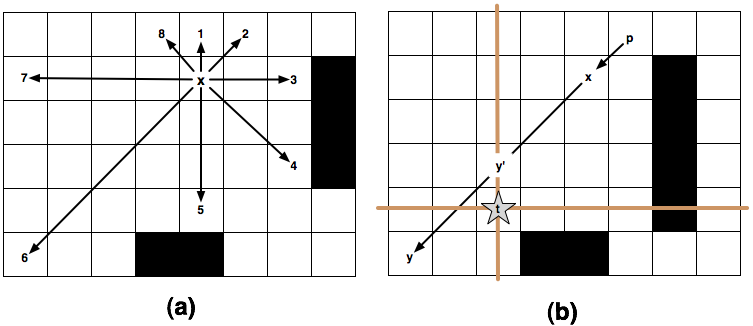
\includegraphics[width=0.95\columnwidth]
			{diagrams/preproc.png}
       \end{center}
	\vspace{-3pt}
       \caption{(a) A jump point is computed in place of each grid neighbour of node $x$.
		the set of neighbours from the grid. (b) In order to reach a jump point $y$ from $x$ it may be
necessary to cross the row or column of the target $t$ (here, both). To make sure we do not jump over 
the target we insert an intermediate successor $y'$ on the row or column of the target (whichever is closest to $x$).}
       \label{fig:preproc}
\end{figure}

The off-line jump points are computed similarly to the on-line jump points 
with the difference that a jump point is defined before each obstacle is hit.  
This addition is necessary 
because the goal state is unknown at preprocessing time.  

At runtime, the algorithm does not need to search for the next jump points 
and can simply find them in the precomputed table.  
Additional tests are however necessary to account for the goal.  

If the current move is a straight move 
and passes over the goal, 
then the jump is stopped at the goal.  

If the current move is a diagonal move 
and crosses the row or the column that contain the goal, 
then a test is performed to check 
whether the goal is visible from the point 
where the jump crosses the line.  
If the goal is indeed visible, 
then the jump is stopped at the crossing point; 
otherwise, the jump continues to the precomputed point.  

On the other hand, the off-line jump point are more numerous 
that the on-line jump point, 
since a jump point is defined even when an obstacle is hit.  
However, it is possible to identify these spurious jump points 
and to avoid inserting them in the queue list.  
DANIEL: YOU PROBABLY WANT TO WRITE SOMETHING ABOUT THIS PARAGRAPH.  
(HOW) DO YOU IDENTIFY THESE SPURIOUS JUMP POINT?  
ARE YOU SURE YOUR IDENTIFICATION PROCEDURE IS CORRECT?  

The benefit of this approach is to remove the computation of the jump point 
and replace it with a simple table lookup.  
The cost of the operation is the additional checks 
presented in the previous paragraphs, 
but it is very limited (much smaller than the gain).  
The preprocessed table induces a limited (linear) memory overhead 
(eight distances for each node in the graph).  
Finally, the preprocessing itself is very low, 
typically in the order of a few seconds.  

I DON'T KNOW WHETHER WE SHOULD MENTION POTENTIAL IMPROVEMENTS HERE.  
FOR INSTANCE, STORING THE TABLE ONLY FROM A JUMP POINT 
(I.E., SEARCH REQUIRED ONLY FOR THE START NODE); 
FILLING THE TABLE DURING THE SEARCH, 
UPDATING THE TABLE WHEN OBSTACLE ARE ADDED/REMOVED.  
